\documentclass[aspectratio=169,12pt]{beamer}

% ─── Theme & Colours ───────────────────────────────────────────────────────────
\usetheme{Madrid}
\usecolortheme{default}
\definecolor{primary}{HTML}{0F2044}
\definecolor{accent}{HTML}{2A9FD6}
\definecolor{light}{HTML}{EAF4FB}
\definecolor{muted}{HTML}{6C7A89}
\definecolor{success}{HTML}{27AE60}
\definecolor{warn}{HTML}{E67E22}

\setbeamercolor{palette primary}{bg=primary,fg=white}
\setbeamercolor{palette secondary}{bg=primary!85,fg=white}
\setbeamercolor{palette tertiary}{bg=primary!70,fg=white}
\setbeamercolor{palette quaternary}{bg=primary,fg=white}
\setbeamercolor{structure}{fg=accent}
\setbeamercolor{block title}{bg=accent,fg=white}
\setbeamercolor{block body}{bg=light,fg=black}
\setbeamercolor{alerted text}{fg=warn}
\setbeamercolor{frametitle}{bg=primary,fg=white}
\setbeamercolor{title}{fg=white}
\setbeamercolor{subtitle}{fg=accent!80}
\setbeamercolor{author}{fg=white!90}
\setbeamercolor{date}{fg=white!70}
\setbeamertemplate{navigation symbols}{}
\setbeamertemplate{footline}[frame number]

% ─── Packages ──────────────────────────────────────────────────────────────────
\usepackage{tikz}
\usetikzlibrary{arrows.meta,shapes.geometric,positioning,fit,backgrounds,decorations.pathreplacing,calc}
\usepackage{fontawesome5}
\usepackage{booktabs}
\usepackage{multicol}
\usepackage{xcolor}
\usepackage{tcolorbox}
\tcbuselibrary{skins,breakable}
\usepackage{pgfplots}
\pgfplotsset{compat=1.18}
\usepackage{array}
\usepackage{adjustbox}

% ─── Custom Boxes ──────────────────────────────────────────────────────────────
\tcbset{
  mybox/.style={
    enhanced,colback=light,colframe=accent,
    boxrule=0.8pt,arc=4pt,left=4pt,right=4pt,top=3pt,bottom=3pt,
    fonttitle=\bfseries\small,attach boxed title to top left={yshift=-2mm,xshift=4mm},
    boxed title style={colback=accent,arc=2pt}
  },
  codebox/.style={
    enhanced,colback=primary!95,colframe=accent,
    boxrule=0.6pt,arc=3pt,left=4pt,right=4pt,top=2pt,bottom=2pt,
    fontupper=\ttfamily\tiny\color{white}
  },
  pillbox/.style={
    enhanced,colback=accent!15,colframe=accent!40,
    boxrule=0.5pt,arc=8pt,left=3pt,right=3pt,top=1pt,bottom=1pt,
    fontupper=\footnotesize\color{primary}\bfseries
  }
}

% ─── TikZ helpers ──────────────────────────────────────────────────────────────
\tikzset{
  pillbox/.style={draw=accent!40,fill=accent!15,rounded corners=8pt,
    inner xsep=5pt,inner ysep=2pt,font=\footnotesize\color{primary}\bfseries,align=center},
  node_box/.style={draw=accent,fill=light,rounded corners=4pt,
    minimum width=1.8cm,minimum height=0.55cm,font=\tiny\bfseries,align=center},
  node_dark/.style={draw=primary,fill=primary,rounded corners=4pt,
    minimum width=1.8cm,minimum height=0.55cm,font=\tiny\bfseries\color{white},align=center},
  node_green/.style={draw=success,fill=success!15,rounded corners=4pt,
    minimum width=1.8cm,minimum height=0.55cm,font=\tiny\bfseries,align=center},
  node_warn/.style={draw=warn,fill=warn!15,rounded corners=4pt,
    minimum width=1.8cm,minimum height=0.55cm,font=\tiny\bfseries,align=center},
  arr/.style={-{Stealth[length=4pt]},draw=accent,thick},
  arr_w/.style={-{Stealth[length=4pt]},draw=white,thick},
}

% ─── Title ─────────────────────────────────────────────────────────────────────
\title{\textbf{Enterprise AI Knowledge Assistant}}
\subtitle{Multi-Tenant RAG SaaS Platform}
\author{Final Year Project Presentation}
\date{2024}
\titlegraphic{\vspace{-10pt}}

% ═══════════════════════════════════════════════════════════════════════════════
\begin{document}
% ═══════════════════════════════════════════════════════════════════════════════

% ── Slide 1 · Cover ────────────────────────────────────────────────────────────
{
\setbeamertemplate{footline}{}
\setbeamercolor{background canvas}{bg=primary}
\begin{frame}[plain]
  \begin{tikzpicture}[remember picture,overlay]
    \fill[accent!20,opacity=0.3] (current page.north west) rectangle ++(16,-2.2);
    \fill[accent,opacity=0.12] (current page.south east) ++(-5,0) rectangle ++(-6,4);
    \foreach \x in {0.4,0.8,...,3.2}{
      \draw[accent!40,ultra thin] (current page.south west) ++(\x,0) -- ++(0,\x*0.6);
    }
    \foreach \y in {0.4,0.8,...,2.4}{
      \draw[accent!30,ultra thin] (current page.south east) ++(0,\y) -- ++(-\y*0.8,0);
    }
    \foreach[count=\i] \tag in {RAG,Multi-Tenant,LangGraph,Vector\,Search,Streaming}{
      \node[pillbox,opacity=0.9] at ($(current page.north east)+(-1.2-\i*2.1,-1.1)$) {\tag};
    }
  \end{tikzpicture}
  \vspace{0.5cm}
  \titlepage
  \vspace{0.2cm}
  \begin{center}
  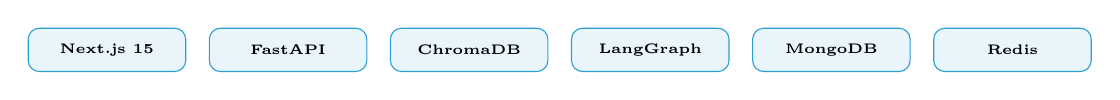
\begin{tikzpicture}
    \foreach[count=\i] \tech in {Next.js 15,FastAPI,ChromaDB,LangGraph,MongoDB,Redis}{
      \node[node_box,minimum width=2cm] at (\i*2.3-6.9,0) {\tech};
    }
  \end{tikzpicture}
  \end{center}
\end{frame}
}

% ── Slide 2 · Agenda ───────────────────────────────────────────────────────────
\begin{frame}{Agenda}
\begin{columns}[T]
\column{0.48\textwidth}
  \begin{tcolorbox}[mybox,title={\faList\; Part I — Problem \& Design}]
    \footnotesize
    \begin{enumerate}
      \item Problem Statement \& Proposed Solution
      \item Technology Stack \& Rationale
      \item High-Level System Architecture
      \item Backend Architecture \& Modules
      \item Authentication \& Authorization Flows
      \item Document Upload \& PDF Pipeline
    \end{enumerate}
  \end{tcolorbox}

\column{0.48\textwidth}
  \begin{tcolorbox}[mybox,title={\faList\; Part II — Core Systems}]
    \footnotesize
    \begin{enumerate}\setcounter{enumi}{6}
      \item Hybrid Retrieval \& LangGraph Workflow
      \item Chat Flow \& Streaming Architecture
      \item Database Schema \& Multi-Tenancy
      \item Frontend Architecture
      \item Security, Performance \& Challenges
      \item Demo Flow \& Future Improvements
      \item Conclusion
    \end{enumerate}
  \end{tcolorbox}
\end{columns}

\vspace{8pt}
\begin{center}
\begin{tikzpicture}
  \foreach[count=\i] \icon/\label in {
    \faCode/Full-Stack,
    \faBrain/AI-Powered,
    \faBuilding/Multi-Tenant,
    \faShieldAlt/Secure,
    \faBolt/Streaming,
    \faSearch/Hybrid RAG}{
    \node[node_box,minimum width=2.2cm] at (\i*2.5-7.5,0) {\icon\\\label};
  }
\end{tikzpicture}
\end{center}
\end{frame}

% ── Slide 3 · Problem → Solution ───────────────────────────────────────────────
\begin{frame}{Problem Statement \& Proposed Solution}
\begin{columns}[T]
\column{0.48\textwidth}
  \begin{tcolorbox}[mybox,title={\faExclamationTriangle\; Problems}]
    \footnotesize
    \begin{itemize}
      \item[\color{warn}$\bullet$] Enterprise knowledge siloed in unstructured PDFs \& docs
      \item[\color{warn}$\bullet$] No context-aware AI search across departments
      \item[\color{warn}$\bullet$] Generic LLMs hallucinate or lack domain knowledge
      \item[\color{warn}$\bullet$] No tenant isolation or role-based access control
      \item[\color{warn}$\bullet$] Costly per-query API calls without caching
      \item[\color{warn}$\bullet$] No audit trail for compliance \& governance
    \end{itemize}
  \end{tcolorbox}
  \vspace{4pt}
  \begin{tcolorbox}[mybox,title={\faBullseye\; Objectives}]
    \footnotesize
    \begin{itemize}
      \item Hybrid retrieval: BM25 + Dense + RRF re-ranking
      \item Multi-tenant isolation per organization/department
      \item Streaming LLM responses via SSE
      \item JWT RBAC with full audit logging
      \item Redis caching \& rate limiting for scale
    \end{itemize}
  \end{tcolorbox}

\column{0.48\textwidth}
  \begin{tcolorbox}[mybox,title={\faLightbulb\; Proposed Solution}]
    \footnotesize
    \textbf{Enterprise AI Knowledge Assistant} — a full-stack, multi-tenant RAG SaaS platform that:
    \vspace{4pt}

    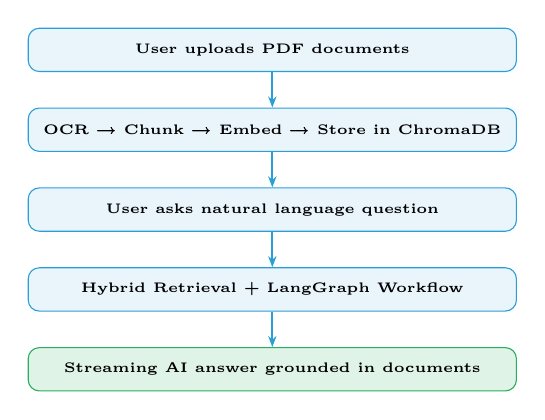
\begin{tikzpicture}[node distance=0.45cm]
      \node[node_box,minimum width=6.2cm] (u) {User uploads PDF documents};
      \node[node_box,minimum width=6.2cm,below=of u] (p) {OCR → Chunk → Embed → Store in ChromaDB};
      \node[node_box,minimum width=6.2cm,below=of p] (q) {User asks natural language question};
      \node[node_box,minimum width=6.2cm,below=of q] (r) {Hybrid Retrieval + LangGraph Workflow};
      \node[node_green,minimum width=6.2cm,below=of r] (a) {Streaming AI answer grounded in documents};
      \draw[arr] (u)--(p); \draw[arr] (p)--(q); \draw[arr] (q)--(r); \draw[arr] (r)--(a);
    \end{tikzpicture}
  \end{tcolorbox}
\end{columns}
\end{frame}

% ── Slide 4 · Technology Stack ─────────────────────────────────────────────────
\begin{frame}{Technology Stack}
\begin{columns}[T]
\column{0.32\textwidth}
  \begin{tcolorbox}[mybox,title={\faReact\; Frontend}]
    \tiny
    \begin{tabular}{@{}ll@{}}
    \textbf{Framework} & Next.js 15 (App Router)\\
    \textbf{Language} & TypeScript\\
    \textbf{Styling} & Tailwind CSS\\
    \textbf{UI} & shadcn/ui\\
    \textbf{State} & Zustand\\
    \textbf{Data Fetch} & TanStack Query\\
    \textbf{HTTP} & Axios\\
    \textbf{Streaming} & Server-Sent Events\\
    \end{tabular}
  \end{tcolorbox}

\column{0.32\textwidth}
  \begin{tcolorbox}[mybox,title={\faPython\; Backend}]
    \tiny
    \begin{tabular}{@{}ll@{}}
    \textbf{Framework} & FastAPI\\
    \textbf{Language} & Python 3.11+\\
    \textbf{AI Workflow} & LangGraph\\
    \textbf{LLM} & Qwen (local)\\
    \textbf{Embeddings} & OpenAI ada-002\\
    \textbf{Auth} & JWT (access + refresh)\\
    \textbf{Email} & SMTP\\
    \textbf{Tasks} & Background Tasks\\
    \end{tabular}
  \end{tcolorbox}

\column{0.32\textwidth}
  \begin{tcolorbox}[mybox,title={\faDatabase\; Data Layer}]
    \tiny
    \begin{tabular}{@{}ll@{}}
    \textbf{Primary DB} & MongoDB\\
    \textbf{Vector DB} & ChromaDB\\
    \textbf{Cache} & Redis\\
    \textbf{Search} & BM25 + Dense\\
    \textbf{Re-rank} & RRF Algorithm\\
    \textbf{PDF} & PyMuPDF / OCR\\
    \textbf{Pattern} & Repository + DI\\
    \textbf{Deploy} & Docker / Cloud\\
    \end{tabular}
  \end{tcolorbox}
\end{columns}

\vspace{6pt}
\begin{tcolorbox}[mybox,title={\faQuestionCircle\; Why These Choices?}]
  \tiny
  \begin{tabular}{@{}p{2.6cm}p{4.2cm}@{\hspace{8pt}}p{2.6cm}p{4.2cm}@{}}
  \textbf{Next.js 15} & App Router + RSC for SSR \& streaming & \textbf{FastAPI} & Async-first, Pydantic validation, OpenAPI auto-docs \\
  \textbf{LangGraph} & Stateful AI workflow as a DAG & \textbf{ChromaDB} & Lightweight, embedded vector search \\
  \textbf{MongoDB} & Flexible schema for multi-tenant docs & \textbf{Redis} & Sub-millisecond cache + atomic rate limiting \\
  \end{tabular}
\end{tcolorbox}
\end{frame}

% ── Slide 5 · High-Level Architecture ──────────────────────────────────────────
\begin{frame}{High-Level System Architecture}
\centering
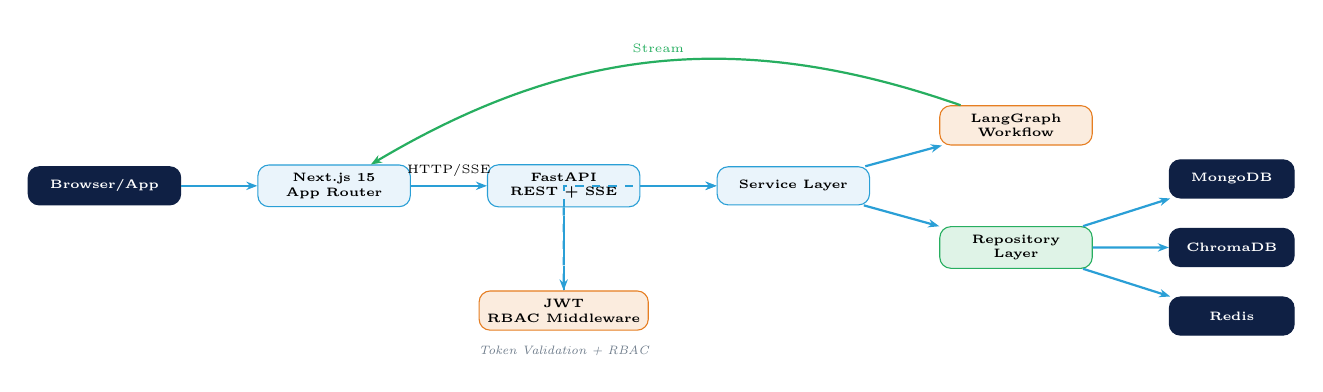
\begin{tikzpicture}[node distance=0.5cm and 0.6cm, scale=0.88, transform shape]

  \node[node_dark,minimum width=2.2cm] (browser) {Browser/App};
  \node[node_box,minimum width=2.2cm, right=1.1cm of browser] (nextjs) {Next.js 15\\App Router};
  \node[node_box,minimum width=2.2cm, right=1.1cm of nextjs] (fastapi) {FastAPI\\REST + SSE};
  \node[node_box,minimum width=2.2cm, right=1.1cm of fastapi] (svc) {Service Layer};
  \node[node_warn,minimum width=2.2cm, above right=0.3cm and 1cm of svc] (lg) {LangGraph\\Workflow};
  \node[node_green,minimum width=2.2cm, below right=0.3cm and 1cm of svc] (repo) {Repository\\Layer};
  \node[node_dark,minimum width=1.8cm, above right=0.4cm and 1.1cm of repo] (mongo) {MongoDB};
  \node[node_dark,minimum width=1.8cm, right=1.1cm of repo] (chroma) {ChromaDB};
  \node[node_dark,minimum width=1.8cm, below right=0.4cm and 1.1cm of repo] (redis) {Redis};
  \node[node_warn,minimum width=2.2cm, below=1.2cm of fastapi] (auth) {JWT\\RBAC Middleware};

  \draw[arr] (browser) -- (nextjs);
  \draw[arr] (nextjs) -- node[above,font=\tiny]{HTTP/SSE} (fastapi);
  \draw[arr] (fastapi) -- (svc);
  \draw[arr] (svc) -- (lg);
  \draw[arr] (svc) -- (repo);
  \draw[arr] (repo) -- (mongo);
  \draw[arr] (repo) -- (chroma);
  \draw[arr] (repo) -- (redis);
  \draw[arr,dashed] (fastapi) -- (auth);
  \draw[arr,dashed] (auth) |- (svc);
  \draw[arr,bend right=25,draw=success] (lg) to node[above,font=\tiny,color=success]{Stream} (nextjs);
  \node[font=\tiny\itshape\color{muted},below=0.1cm of auth] {Token Validation + RBAC};
\end{tikzpicture}

\vspace{6pt}
\begin{columns}[T]
\column{0.24\textwidth}
  \begin{tcolorbox}[pillbox]\centering\faShieldAlt\; JWT + RBAC\end{tcolorbox}
\column{0.24\textwidth}
  \begin{tcolorbox}[pillbox]\centering\faBolt\; SSE Streaming\end{tcolorbox}
\column{0.24\textwidth}
  \begin{tcolorbox}[pillbox]\centering\faBuilding\; Multi-Tenant\end{tcolorbox}
\column{0.24\textwidth}
  \begin{tcolorbox}[pillbox]\centering\faDatabase\; 3-DB Hybrid\end{tcolorbox}
\end{columns}
\end{frame}

% ── Slide 6 · Backend Architecture ─────────────────────────────────────────────
\begin{frame}{Complete Backend Architecture}
\begin{columns}[T]
\column{0.52\textwidth}
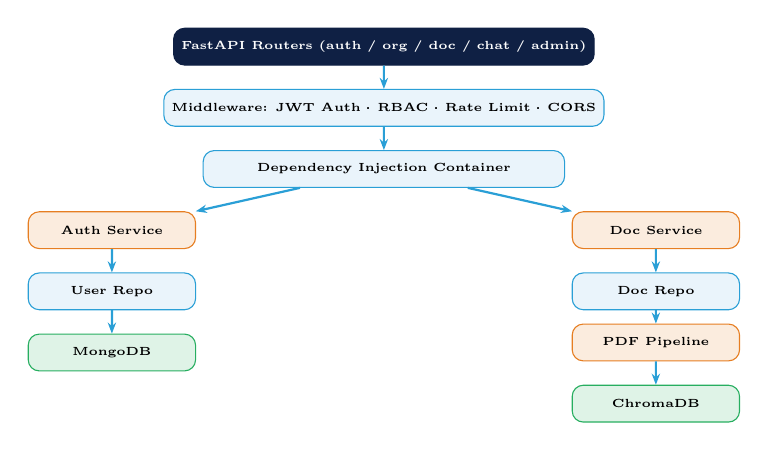
\begin{tikzpicture}[node distance=0.35cm, scale=0.85, transform shape]

  \node[node_dark,minimum width=5.4cm] (router) {FastAPI Routers (auth / org / doc / chat / admin)};
  \node[node_box,minimum width=5.4cm, below=of router] (mid) {Middleware: JWT Auth · RBAC · Rate Limit · CORS};
  \node[node_box,minimum width=5.4cm, below=of mid] (dep) {Dependency Injection Container};

  \node[node_warn,minimum width=2.5cm, below left=0.35cm and 0.1cm of dep] (auth2) {Auth Service};
  \node[node_warn,minimum width=2.5cm, below right=0.35cm and 0.1cm of dep] (doc) {Doc Service};

  \node[node_box,minimum width=2.5cm, below=of auth2] (user_r) {User Repo};
  \node[node_box,minimum width=2.5cm, below=of doc] (doc_r) {Doc Repo};

  \node[node_green,minimum width=2.5cm, below=of user_r] (mg1) {MongoDB};
  \node[node_warn,minimum width=2.5cm, below=0.2cm of doc_r] (pipe) {PDF Pipeline};
  \node[node_green,minimum width=2.5cm, below=of pipe] (chroma2) {ChromaDB};

  \draw[arr] (router)--(mid); \draw[arr] (mid)--(dep);
  \draw[arr] (dep)--(auth2); \draw[arr] (dep)--(doc);
  \draw[arr] (auth2)--(user_r); \draw[arr] (doc)--(doc_r);
  \draw[arr] (user_r)--(mg1); \draw[arr] (doc_r)--(pipe);
  \draw[arr] (pipe)--(chroma2);
\end{tikzpicture}

\column{0.45\textwidth}
  \begin{tcolorbox}[mybox,title={Backend Modules}]
    \tiny
    \textbf{Auth:} JWT login/refresh, signup, email verification, password reset, RBAC\\[3pt]
    \textbf{Organization:} Multi-tenant org \& department CRUD\\[3pt]
    \textbf{Document:} Upload → OCR → Chunk → Embed → ChromaDB\\[3pt]
    \textbf{RAG:} BM25 + Dense + RRF re-rank → LangGraph → Qwen LLM\\[3pt]
    \textbf{Infra:} Redis cache, rate limiting, audit logs, health checks\\[3pt]
    \textbf{Admin:} Dashboard APIs, event logging, snapshot management
  \end{tcolorbox}
  \vspace{4pt}
  \begin{tcolorbox}[mybox,title={Patterns Used}]
    \tiny
    \begin{tabular}{@{}ll@{}}
    Repository Pattern & Abstracts DB layer\\
    Dependency Injection & FastAPI \texttt{Depends()}\\
    Service Layer & Business logic isolation\\
    Event Logging & Full audit trail\\
    Background Tasks & Async PDF processing\\
    \end{tabular}
  \end{tcolorbox}
  \vspace{4pt}
  \begin{tcolorbox}[mybox,title={Folder Structure (Backend)}]
    \tiny
    \begin{tabular}{@{}ll@{}}
    \texttt{/routers} & Endpoint definitions\\
    \texttt{/services} & Business logic\\
    \texttt{/repositories} & DB access layer\\
    \texttt{/models} & Pydantic schemas\\
    \texttt{/core} & Config, DI, security\\
    \texttt{/pipelines} & PDF + embedding flow\\
    \end{tabular}
  \end{tcolorbox}
\end{columns}
\end{frame}

% ── Slide 7 · Auth Flows ───────────────────────────────────────────────────────
\begin{frame}{Authentication \& Authorization Flows}
\begin{columns}[T]
\column{0.48\textwidth}
  \begin{tcolorbox}[mybox,title={\faSignInAlt\; Login / Token Flow}]
  \footnotesize
  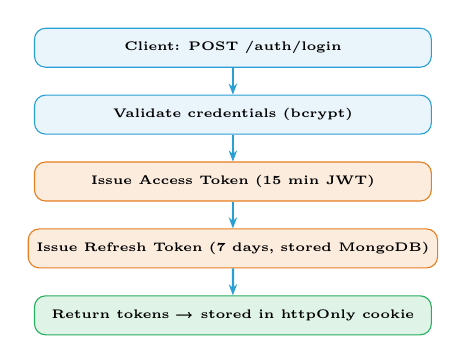
\begin{tikzpicture}[node distance=0.38cm, scale=0.9, transform shape]
    \node[node_box,minimum width=5.6cm] (c) {Client: POST /auth/login};
    \node[node_box,minimum width=5.6cm,below=of c] (v) {Validate credentials (bcrypt)};
    \node[node_warn,minimum width=5.6cm,below=of v] (a) {Issue Access Token (15 min JWT)};
    \node[node_warn,minimum width=5.6cm,below=of a] (r) {Issue Refresh Token (7 days, stored MongoDB)};
    \node[node_green,minimum width=5.6cm,below=of r] (res) {Return tokens → stored in httpOnly cookie};
    \draw[arr](c)--(v);\draw[arr](v)--(a);\draw[arr](a)--(r);\draw[arr](r)--(res);
  \end{tikzpicture}
  \end{tcolorbox}
  \vspace{4pt}
  \begin{tcolorbox}[mybox,title={\faEnvelope\; Email Verification / Password Reset}]
    \tiny
    \textbf{Verification:} Signup → generate token → store in MongoDB → send SMTP link → user clicks → mark verified\\[3pt]
    \textbf{Reset:} Request reset → time-limited token → SMTP → new password → invalidate all sessions\\[3pt]
    \textbf{Signup:} POST /auth/signup → hash password (bcrypt-12) → create user → send verification email
  \end{tcolorbox}

\column{0.48\textwidth}
  \begin{tcolorbox}[mybox,title={\faUserShield\; RBAC \& Multi-Tenant Isolation}]
  \footnotesize
  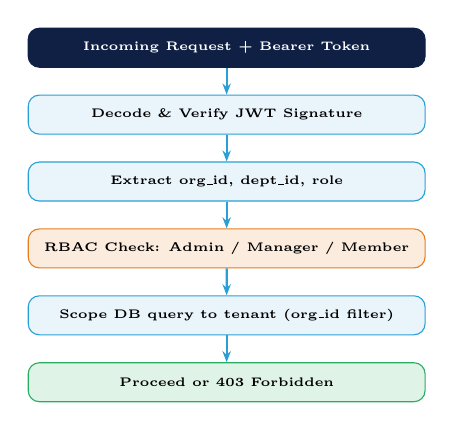
\begin{tikzpicture}[node distance=0.38cm, scale=0.9, transform shape]
    \node[node_dark,minimum width=5.6cm] (req) {Incoming Request + Bearer Token};
    \node[node_box,minimum width=5.6cm,below=of req] (dec) {Decode \& Verify JWT Signature};
    \node[node_box,minimum width=5.6cm,below=of dec] (org) {Extract org\_id, dept\_id, role};
    \node[node_warn,minimum width=5.6cm,below=of org] (rbac) {RBAC Check: Admin / Manager / Member};
    \node[node_box,minimum width=5.6cm,below=of rbac] (scope) {Scope DB query to tenant (org\_id filter)};
    \node[node_green,minimum width=5.6cm,below=of scope] (ok) {Proceed or 403 Forbidden};
    \draw[arr](req)--(dec);\draw[arr](dec)--(org);\draw[arr](org)--(rbac);\draw[arr](rbac)--(scope);\draw[arr](scope)--(ok);
  \end{tikzpicture}
  \end{tcolorbox}
  \vspace{4pt}
  \begin{tcolorbox}[pillbox]\tiny Every MongoDB query filtered by \texttt{org\_id} — tenants are fully isolated at the query level.\end{tcolorbox}
\end{columns}
\end{frame}

% ── Slide 8 · Document Pipeline ────────────────────────────────────────────────
\begin{frame}{Document Upload \& PDF Processing Pipeline}
\vspace{-4pt}
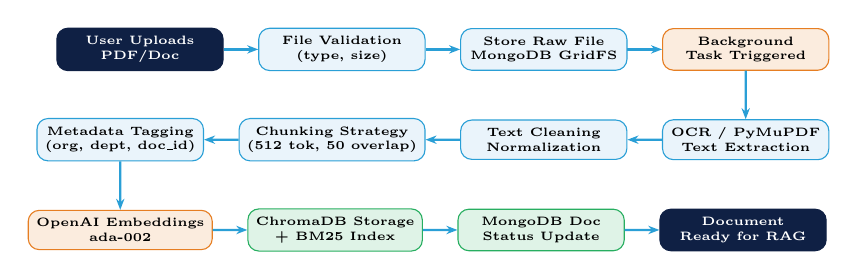
\begin{tikzpicture}[node distance=0.45cm and 0.3cm, scale=0.88, transform shape]

  \node[node_dark,minimum width=2.4cm] (up) {User Uploads\\PDF/Doc};
  \node[node_box,minimum width=2.4cm, right=0.5cm of up] (val) {File Validation\\(type, size)};
  \node[node_box,minimum width=2.4cm, right=0.5cm of val] (store) {Store Raw File\\MongoDB GridFS};
  \node[node_warn,minimum width=2.4cm, right=0.5cm of store] (bg) {Background\\Task Triggered};

  \node[node_box,minimum width=2.4cm, below=0.7cm of bg] (ocr) {OCR / PyMuPDF\\Text Extraction};
  \node[node_box,minimum width=2.4cm, left=0.5cm of ocr] (clean) {Text Cleaning\\Normalization};
  \node[node_box,minimum width=2.4cm, left=0.5cm of clean] (chunk) {Chunking Strategy\\(512 tok, 50 overlap)};
  \node[node_box,minimum width=2.4cm, left=0.5cm of chunk] (meta) {Metadata Tagging\\(org, dept, doc\_id)};

  \node[node_warn,minimum width=2.4cm, below=0.7cm of meta] (emb) {OpenAI Embeddings\\ada-002};
  \node[node_green,minimum width=2.4cm, right=0.5cm of emb] (chroma) {ChromaDB Storage\\+ BM25 Index};
  \node[node_green,minimum width=2.4cm, right=0.5cm of chroma] (mongo2) {MongoDB Doc\\Status Update};
  \node[node_dark,minimum width=2.4cm, right=0.5cm of mongo2] (done) {Document\\Ready for RAG};

  \draw[arr](up)--(val);\draw[arr](val)--(store);\draw[arr](store)--(bg);
  \draw[arr](bg)--(ocr);
  \draw[arr](ocr)--(clean);\draw[arr](clean)--(chunk);\draw[arr](chunk)--(meta);
  \draw[arr](meta)--(emb);
  \draw[arr](emb)--(chroma);\draw[arr](chroma)--(mongo2);\draw[arr](mongo2)--(done);
\end{tikzpicture}

\vspace{6pt}
\begin{columns}[T]
\column{0.32\textwidth}
  \begin{tcolorbox}[mybox,title={Chunking Strategy}]
    \tiny
    Fixed-size: 512 tokens\\
    Overlap: 50 tokens\\
    Preserves sentence boundaries\\
    Recursive text splitter
  \end{tcolorbox}
\column{0.32\textwidth}
  \begin{tcolorbox}[mybox,title={Embedding Model}]
    \tiny
    OpenAI text-embedding-ada-002\\
    1536-dimensional vectors\\
    Batch processing for efficiency\\
    Stored with chunk metadata
  \end{tcolorbox}
\column{0.32\textwidth}
  \begin{tcolorbox}[mybox,title={Background Processing}]
    \tiny
    FastAPI BackgroundTasks\\
    Non-blocking upload response\\
    Status: pending → processing → ready\\
    Error handling \& retry logic
  \end{tcolorbox}
\end{columns}
\end{frame}

% ── Slide 9 · Retrieval Pipeline ───────────────────────────────────────────────
\begin{frame}{Hybrid Retrieval Pipeline \& LangGraph Workflow}
\begin{columns}[T]
\column{0.50\textwidth}
  \textbf{\color{primary}Hybrid Retrieval Architecture}
  \vspace{4pt}

  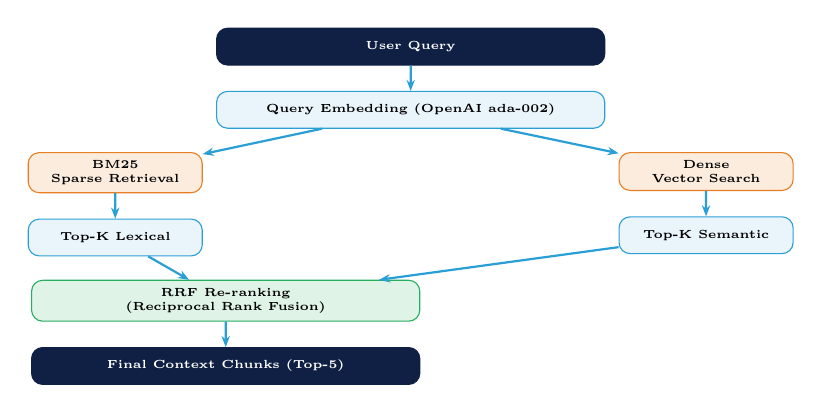
\begin{tikzpicture}[node distance=0.38cm, scale=0.85, transform shape]
    \node[node_dark,minimum width=5.8cm] (q) {User Query};
    \node[node_box,minimum width=5.8cm,below=of q] (qe) {Query Embedding (OpenAI ada-002)};

    \node[node_warn,minimum width=2.6cm, below left=0.35cm and 0.2cm of qe] (bm25) {BM25\\Sparse Retrieval};
    \node[node_warn,minimum width=2.6cm, below right=0.35cm and 0.2cm of qe] (dense) {Dense\\Vector Search};

    \node[node_box,minimum width=2.6cm,below=of bm25] (r1) {Top-K Lexical};
    \node[node_box,minimum width=2.6cm,below=of dense] (r2) {Top-K Semantic};

    \node[node_green,minimum width=5.8cm,below=0.35cm of r1,xshift=1.65cm] (rrf) {RRF Re-ranking\\(Reciprocal Rank Fusion)};
    \node[node_dark,minimum width=5.8cm,below=of rrf] (ctx) {Final Context Chunks (Top-5)};

    \draw[arr](q)--(qe);
    \draw[arr](qe)--(bm25);\draw[arr](qe)--(dense);
    \draw[arr](bm25)--(r1);\draw[arr](dense)--(r2);
    \draw[arr](r1)--(rrf);\draw[arr](r2)--(rrf);
    \draw[arr](rrf)--(ctx);
  \end{tikzpicture}

\column{0.47\textwidth}
  \textbf{\color{primary}LangGraph Workflow (DAG)}
  \vspace{4pt}

  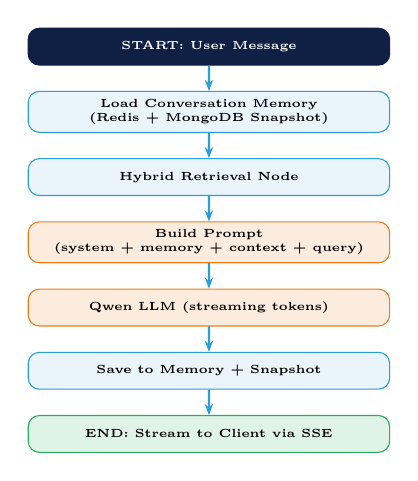
\begin{tikzpicture}[node distance=0.38cm, scale=0.85, transform shape]
    \node[node_dark,minimum width=5.4cm] (start) {START: User Message};
    \node[node_box,minimum width=5.4cm,below=of start] (mem) {Load Conversation Memory\\(Redis + MongoDB Snapshot)};
    \node[node_box,minimum width=5.4cm,below=of mem] (ret) {Hybrid Retrieval Node};
    \node[node_warn,minimum width=5.4cm,below=of ret] (prompt) {Build Prompt\\(system + memory + context + query)};
    \node[node_warn,minimum width=5.4cm,below=of prompt] (llm) {Qwen LLM (streaming tokens)};
    \node[node_box,minimum width=5.4cm,below=of llm] (save) {Save to Memory + Snapshot};
    \node[node_green,minimum width=5.4cm,below=of save] (end) {END: Stream to Client via SSE};

    \draw[arr](start)--(mem);\draw[arr](mem)--(ret);\draw[arr](ret)--(prompt);
    \draw[arr](prompt)--(llm);\draw[arr](llm)--(save);\draw[arr](save)--(end);
  \end{tikzpicture}
\end{columns}
\end{frame}

% ── Slide 10 · Streaming Chat ──────────────────────────────────────────────────
\begin{frame}{Chat Flow \& Streaming Response Architecture}
\vspace{-2pt}
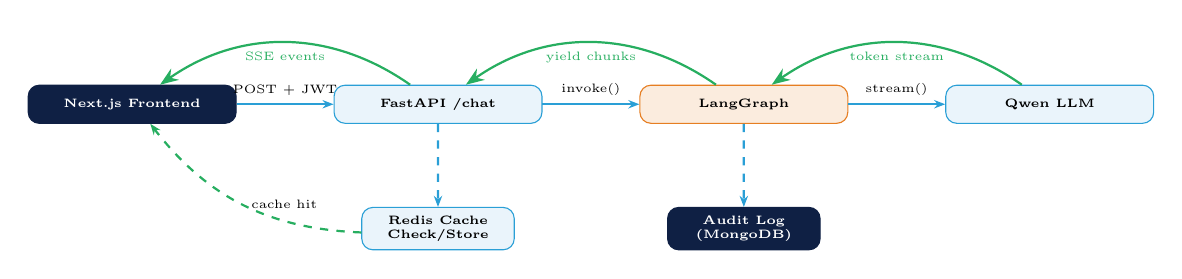
\begin{tikzpicture}[node distance=0.42cm and 0.5cm, scale=0.88, transform shape]

  \node[node_dark,minimum width=3cm] (fe) {Next.js Frontend};
  \node[node_box,minimum width=3cm, right=1.4cm of fe] (api) {FastAPI /chat};
  \node[node_warn,minimum width=3cm, right=1.4cm of api] (lg2) {LangGraph};
  \node[node_box,minimum width=3cm, right=1.4cm of lg2] (qwen) {Qwen LLM};

  \draw[arr] (fe) -- node[above,font=\tiny]{POST + JWT} (api);
  \draw[arr] (api) -- node[above,font=\tiny]{invoke()} (lg2);
  \draw[arr] (lg2) -- node[above,font=\tiny]{stream()} (qwen);

  \draw[-{Stealth},draw=success,thick] (qwen) to[bend right=35]
    node[below,font=\tiny,color=success]{token stream} (lg2);
  \draw[-{Stealth},draw=success,thick] (lg2) to[bend right=35]
    node[below,font=\tiny,color=success]{yield chunks} (api);
  \draw[-{Stealth},draw=success,thick] (api) to[bend right=35]
    node[below,font=\tiny,color=success]{SSE events} (fe);

  \node[node_box,minimum width=2.2cm, below=1.2cm of api] (redis2) {Redis Cache\\Check/Store};
  \draw[arr,dashed] (api) -- (redis2);
  \draw[arr,dashed,draw=success] (redis2) to[bend left=25] node[right,font=\tiny]{cache hit} (fe);

  \node[node_dark,minimum width=2.2cm, below=1.2cm of lg2] (audit) {Audit Log\\(MongoDB)};
  \draw[arr,dashed] (lg2) -- (audit);
\end{tikzpicture}

\vspace{6pt}
\begin{columns}[T]
\column{0.32\textwidth}
  \begin{tcolorbox}[mybox,title={SSE Streaming}]
    \tiny
    FastAPI \texttt{StreamingResponse}\\
    Yields: \texttt{data: \{token\}\textbackslash n\textbackslash n}\\
    Frontend: \texttt{EventSource} API\\
    TanStack Query manages state\\
    Zustand accumulates tokens
  \end{tcolorbox}
\column{0.32\textwidth}
  \begin{tcolorbox}[mybox,title={Conversation Memory}]
    \tiny
    Short-term: Redis (last N turns)\\
    Long-term: MongoDB snapshots\\
    Snapshot trigger: every 20 msgs\\
    Summarized by LLM to save tokens\\
    Multi-session persistence
  \end{tcolorbox}
\column{0.32\textwidth}
  \begin{tcolorbox}[mybox,title={Rate Limiting}]
    \tiny
    Redis atomic counter per user\\
    Sliding window algorithm\\
    Limits: msgs/min, docs/day\\
    429 Too Many Requests response\\
    Admin override capability
  \end{tcolorbox}
\end{columns}
\end{frame}

% ── Slide 11 · Database Schema ─────────────────────────────────────────────────
\begin{frame}{Database Schema \& Multi-Tenant Architecture}
\begin{columns}[T]
\column{0.52\textwidth}
  \textbf{\color{primary}MongoDB Collections}
  \vspace{4pt}

  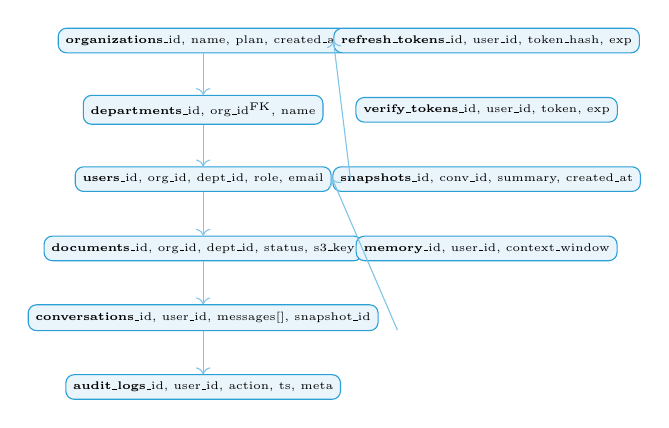
\begin{tikzpicture}[scale=0.8, transform shape,
    entity/.style={draw=accent,fill=light,rounded corners=3pt,minimum width=3.2cm,font=\tiny},
    field/.style={font=\tiny,text=muted}]

    \node[entity] (org) at (0,4.2) {\textbf{organizations}\\\_id, name, plan, created\_at};
    \node[entity] (dept) at (0,3.1) {\textbf{departments}\\\_id, org\_id\textsuperscript{FK}, name};
    \node[entity] (user) at (0,2.0) {\textbf{users}\\\_id, org\_id, dept\_id, role, email};
    \node[entity] (doc) at (0,0.9) {\textbf{documents}\\\_id, org\_id, dept\_id, status, s3\_key};
    \node[entity] (conv) at (0,-0.2) {\textbf{conversations}\\\_id, user\_id, messages[], snapshot\_id};
    \node[entity] (audit) at (0,-1.3) {\textbf{audit\_logs}\\\_id, user\_id, action, ts, meta};
    \node[entity] (tok) at (4.5,4.2) {\textbf{refresh\_tokens}\\\_id, user\_id, token\_hash, exp};
    \node[entity] (ver) at (4.5,3.1) {\textbf{verify\_tokens}\\\_id, user\_id, token, exp};
    \node[entity] (snap) at (4.5,2.0) {\textbf{snapshots}\\\_id, conv\_id, summary, created\_at};
    \node[entity] (mem) at (4.5,0.9) {\textbf{memory}\\\_id, user\_id, context\_window};

    \draw[draw=accent!60,->] (org.south)--(dept.north);
    \draw[draw=accent!60,->] (dept.south)--(user.north);
    \draw[draw=accent!60,->] (user.south)--(doc.north);
    \draw[draw=accent!60,->] (doc.south)--(conv.north);
    \draw[draw=accent!60,->] (conv.south)--(audit.north);
    \draw[draw=accent!60,->] ($(user.east) + (0.3,0)$) -- (tok.west);
    \draw[draw=accent!60,->] ($(conv.east) + (0.3,-0.2)$) -- (snap.west);
  \end{tikzpicture}

\column{0.44\textwidth}
  \begin{tcolorbox}[mybox,title={ChromaDB Collections}]
    \tiny
    \textbf{Collection per org/dept:}\\
    \texttt{org\_\{id\}\_dept\_\{id\}\_docs}\\[4pt]
    Each document stored as:\\
    \begin{tabular}{@{}ll@{}}
    \texttt{id} & chunk UUID\\
    \texttt{embedding} & 1536-dim vector\\
    \texttt{metadata} & \{doc\_id, chunk\_n, text\}\\
    \end{tabular}\\[4pt]
    Tenant isolation: separate collection namespaces
  \end{tcolorbox}
  \vspace{4pt}
  \begin{tcolorbox}[mybox,title={Redis Keys}]
    \tiny
    \begin{tabular}{@{}ll@{}}
    \texttt{cache:\{hash\}} & Query result cache\\
    \texttt{rl:\{uid\}:min} & Rate limit counter\\
    \texttt{session:\{uid\}} & Active session\\
    \texttt{memory:\{uid\}} & Short-term context\\
    \end{tabular}\\[4pt]
    TTLs: cache=1h, rate=60s, session=15m
  \end{tcolorbox}
  \vspace{4pt}
  \begin{tcolorbox}[pillbox]\tiny All DB queries scoped by \texttt{org\_id} — zero cross-tenant data leakage.\end{tcolorbox}
\end{columns}
\end{frame}

% ── Slide 12 · Frontend Architecture ──────────────────────────────────────────
\begin{frame}{Frontend Architecture}
\begin{columns}[T]
\column{0.50\textwidth}
  \textbf{\color{primary}Next.js 15 App Router Structure}
  \vspace{4pt}

  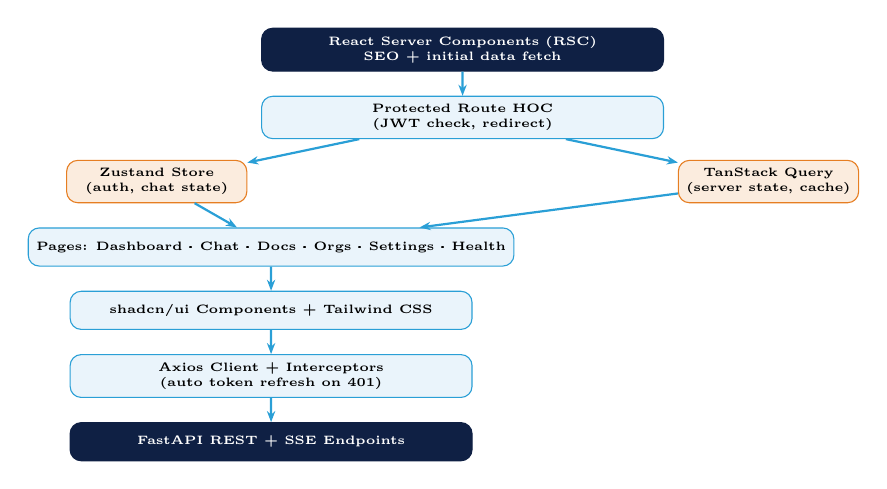
\begin{tikzpicture}[node distance=0.35cm, scale=0.88, transform shape]
    \node[node_dark,minimum width=5.8cm] (rsc) {React Server Components (RSC)\\SEO + initial data fetch};
    \node[node_box,minimum width=5.8cm,below=of rsc] (prot) {Protected Route HOC\\(JWT check, redirect)};

    \node[node_warn,minimum width=2.6cm, below left=0.3cm and 0.2cm of prot] (z) {Zustand Store\\(auth, chat state)};
    \node[node_warn,minimum width=2.6cm, below right=0.3cm and 0.2cm of prot] (tq) {TanStack Query\\(server state, cache)};

    \node[node_box,minimum width=5.8cm, below=0.35cm of z,xshift=1.65cm] (pages) {Pages: Dashboard · Chat · Docs · Orgs · Settings · Health};
    \node[node_box,minimum width=5.8cm,below=of pages] (comp) {shadcn/ui Components + Tailwind CSS};
    \node[node_box,minimum width=5.8cm,below=of comp] (axios) {Axios Client + Interceptors\\(auto token refresh on 401)};
    \node[node_dark,minimum width=5.8cm,below=of axios] (api2) {FastAPI REST + SSE Endpoints};

    \draw[arr](rsc)--(prot); \draw[arr](prot)--(z); \draw[arr](prot)--(tq);
    \draw[arr](z)--(pages); \draw[arr](tq)--(pages);
    \draw[arr](pages)--(comp); \draw[arr](comp)--(axios); \draw[arr](axios)--(api2);
  \end{tikzpicture}

\column{0.46\textwidth}
  \begin{tcolorbox}[mybox,title={State Management}]
    \tiny
    \textbf{Zustand} — global client state:\\
    auth slice (user, tokens, org),\\
    chat slice (messages, streaming),\\
    ui slice (sidebar, modals)\\[4pt]
    \textbf{TanStack Query} — server state:\\
    documents, organizations, departments;\\
    background refetch + stale-while-revalidate
  \end{tcolorbox}
  \vspace{4pt}
  \begin{tcolorbox}[mybox,title={Streaming Chat UI}]
    \tiny
    Open \texttt{EventSource} → \texttt{/chat/stream}\\
    On \texttt{message}: append token to Zustand\\
    On \texttt{done}: mark message complete\\
    Abort controller for cancel-stream\\
    Loading skeleton during first token
  \end{tcolorbox}
  \vspace{4pt}
  \begin{tcolorbox}[mybox,title={Frontend Folder Structure}]
    \tiny
    \begin{tabular}{@{}ll@{}}
    \texttt{/app} & App Router pages \& layouts\\
    \texttt{/components} & shadcn/ui + custom\\
    \texttt{/store} & Zustand slices\\
    \texttt{/hooks} & TanStack Query hooks\\
    \texttt{/lib} & Axios client, utils\\
    \texttt{/types} & TypeScript interfaces\\
    \end{tabular}
  \end{tcolorbox}
\end{columns}
\end{frame}

% ── Slide 13 · Security, Performance, Challenges & Conclusion ──────────────────
\begin{frame}{Security · Performance · Challenges · Demo · Future}
\begin{columns}[T]
\column{0.32\textwidth}
  \begin{tcolorbox}[mybox,title={\faShieldAlt\; Security Features}]
    \tiny
    \begin{itemize}
      \item bcrypt password hashing (cost 12)
      \item httpOnly cookies for refresh tokens
      \item JWT RS256 with key rotation
      \item CORS whitelist + CSP headers
      \item Input sanitisation (Pydantic)
      \item RBAC at service + query level
      \item Org-scoped DB queries
      \item SMTP TLS for all emails
      \item Rate limiting (Redis)
      \item Full audit log every action
    \end{itemize}
  \end{tcolorbox}

\column{0.32\textwidth}
  \begin{tcolorbox}[mybox,title={\faBolt\; Performance Optimizations}]
    \tiny
    \begin{itemize}
      \item Redis cache (1h TTL) for RAG results
      \item Async FastAPI throughout
      \item Background task for PDF processing
      \item Chunked streaming (no wait for full LLM)
      \item TanStack Query stale-while-revalidate
      \item MongoDB compound indexes on org\_id
      \item ChromaDB HNSW approximate NN
      \item BM25 inverted index for lexical speed
      \item Connection pooling (MongoDB Motor)
    \end{itemize}
  \end{tcolorbox}

\column{0.32\textwidth}
  \begin{tcolorbox}[mybox,title={\faTools\; Challenges \& Solutions}]
    \tiny
    \textbf{Challenge 1:} SSE + JWT auth\\
    \textit{Solution:} Token in query param, validated at handshake\\[3pt]
    \textbf{Challenge 2:} Multi-tenant data isolation\\
    \textit{Solution:} Middleware injects org\_id into every repo call\\[3pt]
    \textbf{Challenge 3:} LLM hallucinations\\
    \textit{Solution:} Grounded prompts — ``Answer ONLY from context''\\[3pt]
    \textbf{Challenge 4:} Large PDF processing blocking\\
    \textit{Solution:} BackgroundTasks + status polling\\[3pt]
    \textbf{Challenge 5:} Context window limits\\
    \textit{Solution:} Snapshot + summarization at 20 msgs
  \end{tcolorbox}
\end{columns}

\vspace{4pt}
\begin{columns}[T]
\column{0.48\textwidth}
  \begin{tcolorbox}[mybox,title={\faPlayCircle\; Demo Flow}]
    \tiny
    \begin{enumerate}
      \item Signup → Email Verification → Login
      \item Create Organization \& Department
      \item Upload PDF → Watch processing status
      \item Ask natural-language question
      \item Observe streaming AI response + citations
      \item Admin: view audit logs \& rate limits
    \end{enumerate}
  \end{tcolorbox}
\column{0.48\textwidth}
  \begin{tcolorbox}[mybox,title={\faRocket\; Future Improvements}]
    \tiny
    \begin{tabular}{@{}p{3.8cm}p{3.8cm}@{}}
    Fine-tune Qwen on domain data & GraphQL subscriptions for real-time\\
    Kubernetes auto-scaling & Mobile app (React Native)\\
    Automated testing suite (pytest) & CI/CD pipeline (GitHub Actions)\\
    \end{tabular}
  \end{tcolorbox}
\end{columns}
\end{frame}

% ── Slide (End) · Conclusion & Thank You ──────────────────────────────────────
{
\setbeamercolor{background canvas}{bg=primary}
\setbeamertemplate{footline}{}
\begin{frame}[plain]
\begin{tikzpicture}[remember picture,overlay]
  \fill[accent!15,opacity=0.3] (current page.north west) rectangle ++(16,-2);
  \fill[accent,opacity=0.1] (current page.south east) ++(-4,0) rectangle ++(-7,3.5);
\end{tikzpicture}

\vspace{0.5cm}
{\Large\bfseries\color{white}Conclusion}\\[8pt]
{\color{accent!80}\rule{0.6\textwidth}{0.8pt}}\\[12pt]

\begin{columns}[T]
\column{0.55\textwidth}
  \begin{tcolorbox}[enhanced,colback=white!8,colframe=accent!50,arc=4pt,boxrule=0.6pt]
  \small\color{white}
  \begin{itemize}
    \item[\color{accent}$\checkmark$] Full-stack enterprise RAG SaaS — production-ready architecture
    \item[\color{accent}$\checkmark$] Hybrid retrieval (BM25 + Dense + RRF) for superior answer quality
    \item[\color{accent}$\checkmark$] Multi-tenant isolation with JWT RBAC and full audit trail
    \item[\color{accent}$\checkmark$] Real-time streaming responses via SSE + LangGraph DAG
    \item[\color{accent}$\checkmark$] Redis caching and rate limiting for enterprise-scale performance
    \item[\color{accent}$\checkmark$] Repository pattern + DI for clean, testable, maintainable code
  \end{itemize}
  \end{tcolorbox}

\column{0.40\textwidth}
  \vspace{4pt}
  \begin{tcolorbox}[enhanced,colback=white!8,colframe=accent!50,arc=4pt,boxrule=0.6pt]
  \centering\color{white}
  \textbf{\color{accent}Tech at a Glance}\\[6pt]
  \footnotesize
  \begin{tabular}{@{}ll@{}}
  \faCode & Next.js 15 + FastAPI\\
  \faBrain & LangGraph + Qwen LLM\\
  \faSearch & BM25 + Dense + RRF\\
  \faDatabase & Mongo + Chroma + Redis\\
  \faShieldAlt & JWT + RBAC + Audit\\
  \faBolt & SSE Streaming + Cache\\
  \end{tabular}
  \end{tcolorbox}
\end{columns}

\vspace{0.6cm}
\begin{center}
  {\Huge\color{accent}\faHandshake}\\[4pt]
  {\large\bfseries\color{white}Thank You}\\[4pt]
  {\footnotesize\color{white!70}Questions \& Discussion Welcome}
\end{center}
\end{frame}
}

\end{document}